\section{Resultados}
\label{sec:resultados}

Os resultados correspondem ao cenário ambiental exploratório descrito na seção~\ref{sec:dados}.

\subsection{Contas ambientais, volume e concentração}

As duas contas totalizam 683,70 mil Gg de CO\textsubscript{2}, dos quais 392,92 mil Gg estão na diagonal de $F$ e 290,78 mil Gg nas relações entre atividades distintas em $W$. A igualdade entre os totais pela produção e pela demanda decorre da identidade contábil.

A rede completa tem 67 nós e 4\,290 arestas, com densidade de 97,01\%. Serviços domésticos (9700) é o único isolado: sua conta permanece na diagonal de $F$. As outras 66 atividades estão ligadas entre si nas duas direções, com graus iguais a 65. O número de ligações pouco distingue os perfis setoriais.

Os pesos, entretanto, distinguem volume e concentração (Figura~\ref{fig:indicadores-resultados}). Energia (3500) e água, esgoto e resíduos (3680) distribuem volumes externos próximos, de 31,32 e 31,23 mil Gg, mas apresentam 20,79 e 9,88 destinos efetivos. Assim, o volume de energia é mais distribuído entre contrapartes, enquanto o de água e resíduos é mais concentrado.

Energia e construção ocupam posições distintas nas contas completas (Tabela~\ref{tab:contas-energia-construcao}). Em energia, a produção supera a atribuição pela demanda; em construção ocorre o inverso. A pequena saída intersetorial de construção não indica baixa emissão própria: a maior parte de sua conta pela produção é atribuída à demanda final da própria atividade e permanece fora de $W$.

\clearpage
\begin{table}[!ht]
\centering
\caption{Contas e volumes intersetoriais de energia e construção.}
\label{tab:contas-energia-construcao}
\small
\begin{tabular}{@{}lrr@{}}
\toprule
Medida & Energia (3500) & Construção (4180) \\
\midrule
Produção, $c$ & 56,62 & 38,84 \\
Demanda, $u$ & 28,23 & 59,40 \\
Atribuição à própria atividade, $F_{ii}$ & 25,30 & 35,91 \\
Saída externa, $s^{\mathrm{out}}$ & 31,32 & 2,93 \\
Entrada externa, $s^{\mathrm{in}}$ & 2,92 & 23,48 \\
Saldo, $u-c$ & $-28,39$ & 20,56 \\
\bottomrule
\end{tabular}
\par\smallskip\begin{minipage}{\textwidth}\footnotesize
Fonte: elaboração própria. Valores em mil Gg de CO\textsubscript{2}, antes do filtro. A diagonal integra $c$ e $u$, mas não as forças externas. Diferenças residuais entre somas de valores exibidos decorrem do arredondamento.
\end{minipage}
\end{table}



\subsection{Seleção das relações e limites de cobertura}

O backbone de referência preserva 575 arestas, ou 13,40\% das ligações de $W$, e 70,69\% do peso intersetorial (Tabela~\ref{tab:sensibilidade-backbone}). Os painéis da Figura~\ref{fig:matriz-backbone} distinguem presença e peso: nem todas as ligações retidas correspondem a grandes volumes absolutos.

\begin{table}[htbp]
\centering
\caption{Sensibilidade da seleção e da cobertura ao parâmetro do filtro.}
\label{tab:sensibilidade-backbone}
\small
\begin{tabular}{@{}crrrr@{}}
\toprule
$\alpha$ & Arestas & \% das arestas de $W$ & Peso retido & Cobertura (\%) \\
\midrule
0,01 & 338 & 7,88 & 166,88 & 57,39 \\
0,05 & 575 & 13,40 & 205,55 & 70,69 \\
0,10 & 755 & 17,60 & 224,92 & 77,35 \\
\bottomrule
\end{tabular}
\par\smallskip\begin{minipage}{\textwidth}\footnotesize
Fonte: elaboração própria. Peso em mil Gg de CO\textsubscript{2}. Cobertura relativa ao peso de $W$, sem diagonal. Todos os casos mantêm 67 nós, um isolado e um componente fracamente conectado de 66 atividades. O filtro é aplicado à mesma rede completa, com regra OU e sem atualização dos perfis.
\end{minipage}
\end{table}

A cobertura agregada oculta perdas locais. Em $\alpha=0{,}05$, as menores coberturas são 32,96\% nas saídas e 33,79\% nas entradas. Portanto, preservar parcela expressiva do peso total não assegura representação igualmente completa de cada atividade e direção.

A mudança de $\alpha$ altera as posições individuais por grau, embora o componente de 66 atividades permaneça nos três casos. A conectividade agregada não demonstra estabilidade das posições setoriais. Os valores detalhados das mudanças e a decomposição da seleção por extremidade constam do Anexo~\ref{anexo:diagnosticos}; $0{,}05$ permanece como referência, sem ser considerado um parâmetro ótimo.



\clearpage
\newgeometry{margin=1.5cm}
\begin{landscape}
\begin{figure}[p]
\centering
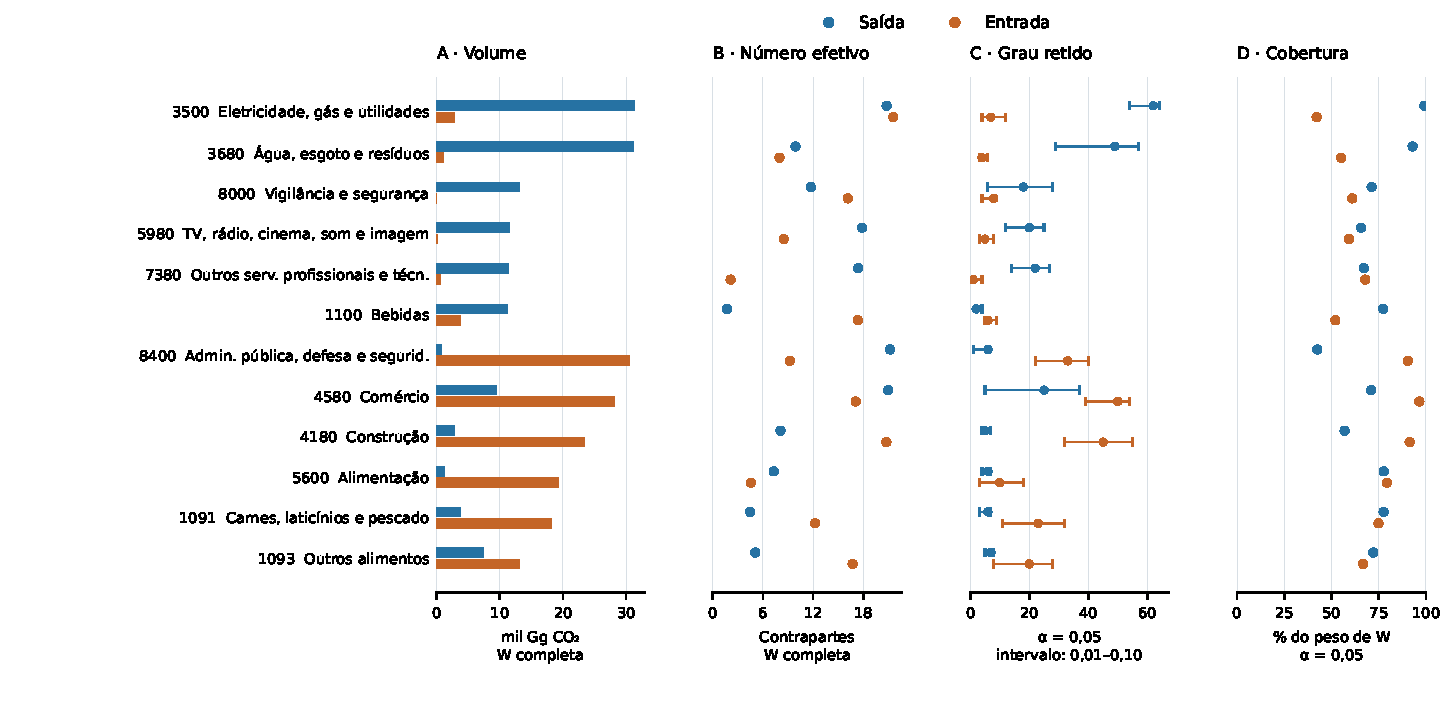
\includegraphics[width=\linewidth,height=0.80\textheight,keepaspectratio]{figuras/indicadores.pdf}
\caption{Volume, concentração, conectividade selecionada e cobertura em atividades de maior volume externo.}
\label{fig:indicadores-resultados}
\begin{minipage}{\linewidth}\footnotesize
Fonte: elaboração própria. Linhas: união das seis maiores forças de saída e das seis maiores forças de entrada de $W$; não representam todas as atividades. Azul: saída; laranja: entrada. Volume e número efetivo são calculados em $W$ completa. Grau e cobertura referem-se a $\alpha=0{,}05$; os intervalos do grau abrangem $\alpha=0{,}01$--$0{,}10$ e não são intervalos de confiança. A diagonal é excluída.
\end{minipage}
\end{figure}
\end{landscape}
\restoregeometry

\clearpage
\newgeometry{margin=1.5cm}
\begin{landscape}
\begin{figure}[p]
\centering
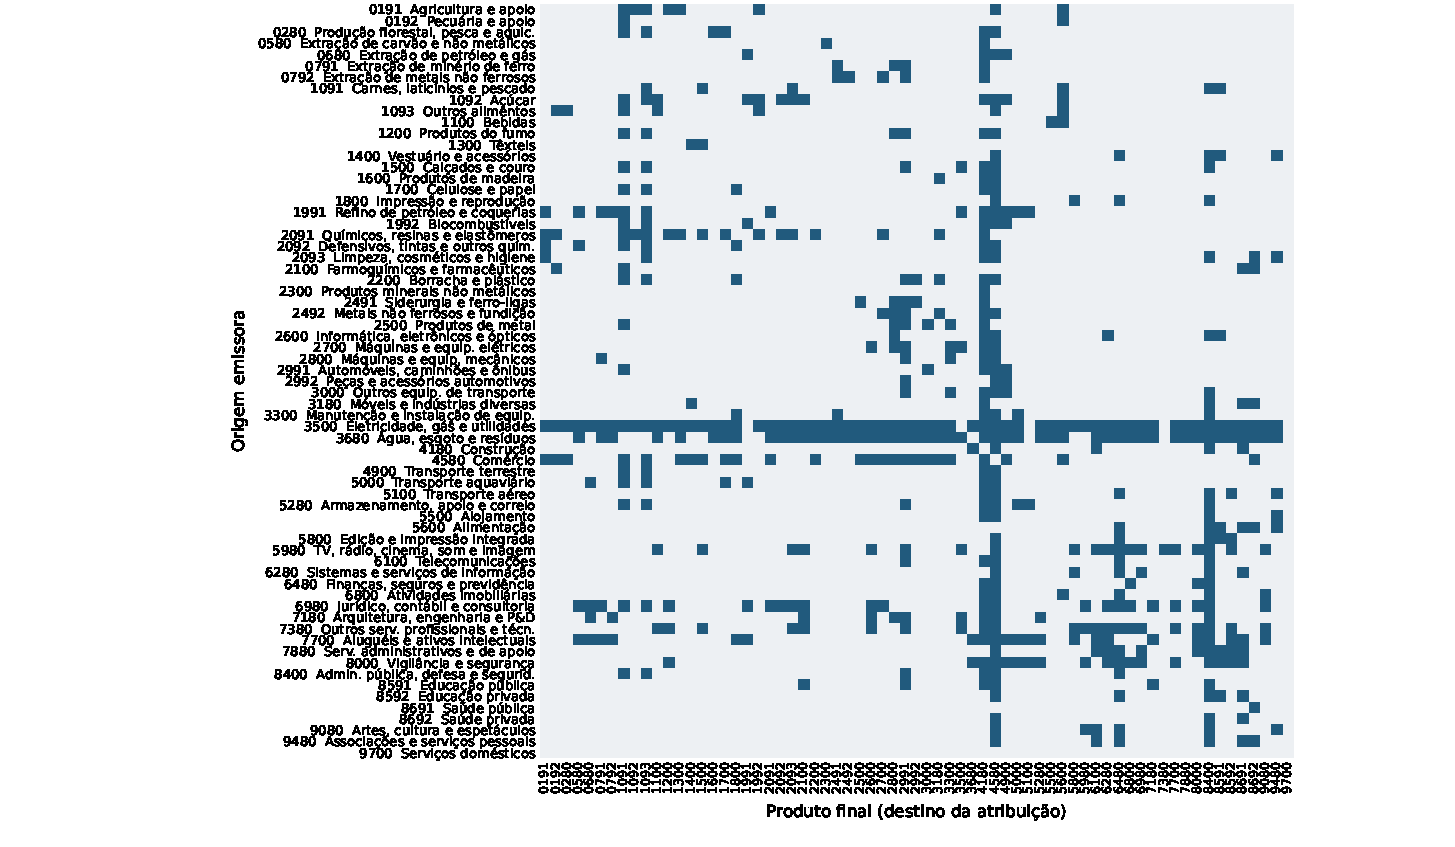
\includegraphics[width=\linewidth,height=0.82\textheight,keepaspectratio]{figuras/matriz_presenca.pdf}
\caption{Matriz de adjacência do backbone com $\alpha=0{,}05$: (a) presença das arestas.}
\label{fig:matriz-backbone}
\begin{minipage}{\linewidth}\footnotesize
Fonte: elaboração própria. Linha: origem emissora; coluna: atividade do produto final. Ordem setorial do IBGE nos dois eixos. Azul identifica as 575 ligações retidas; cinza indica ausência no backbone, inclusive a diagonal. Ausência no backbone não implica valor nulo em $F$ ou $W$. Todas as 67 atividades permanecem nos eixos.
\end{minipage}
\end{figure}
\clearpage
\begin{figure}[p]
\ContinuedFloat
\centering
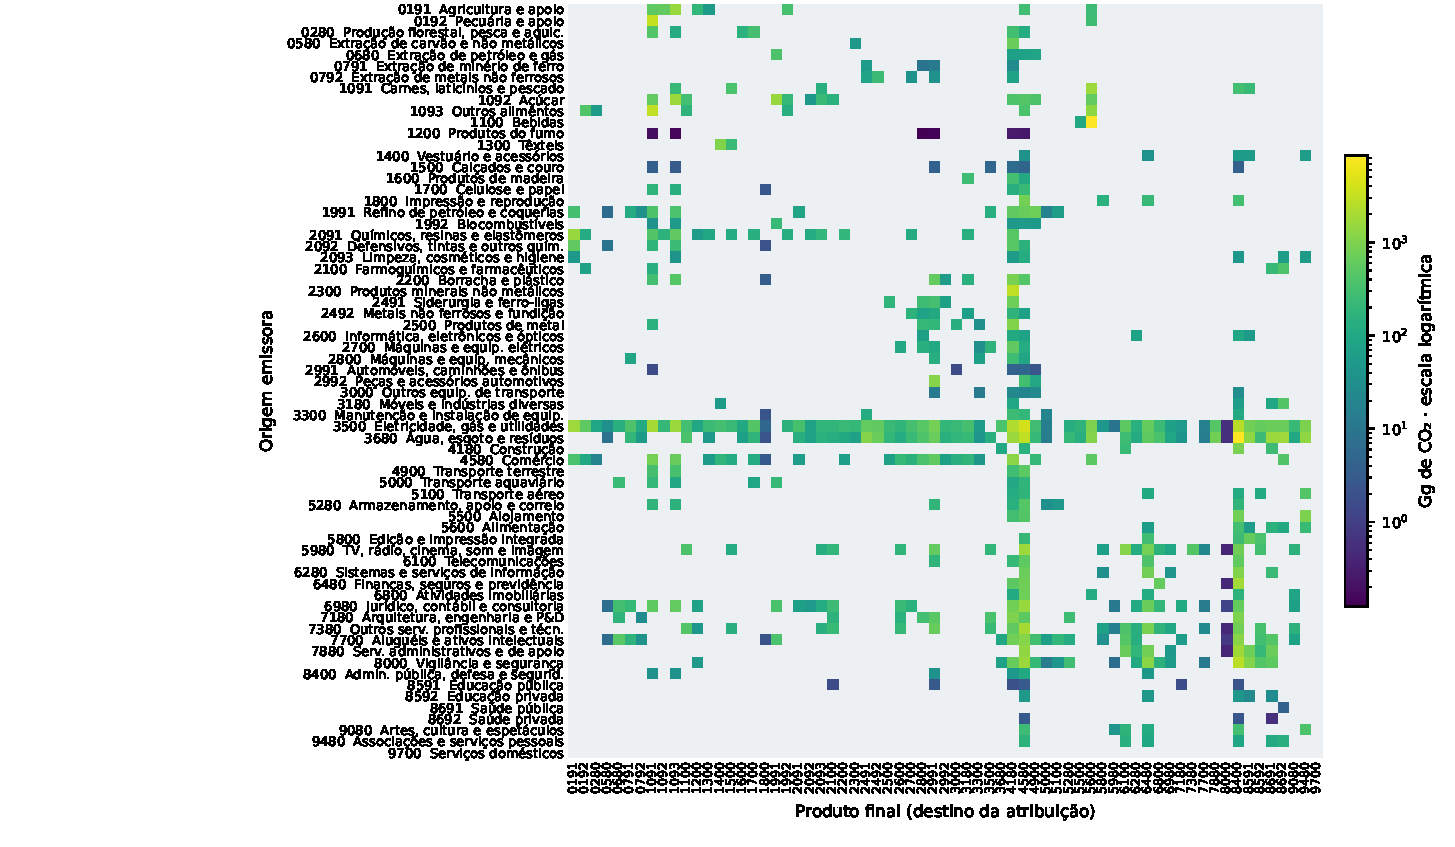
\includegraphics[width=\linewidth,height=0.82\textheight,keepaspectratio]{figuras/matriz_peso.pdf}
\caption{Matriz de adjacência do backbone com $\alpha=0{,}05$: (b) pesos das mesmas arestas.}
\begin{minipage}{\linewidth}\footnotesize
Fonte: elaboração própria. Mesma ordem e mesma seleção do painel (a). A cor representa pesos originais em Gg de CO\textsubscript{2}, em escala logarítmica, sem normalização por linha ou coluna. Cinza identifica células sem aresta retida. A cor mede volume absoluto; a concentração é descrita pelos números efetivos em $W$ completa.
\end{minipage}
\end{figure}
\end{landscape}
\restoregeometry

\subsection{Energia e construção: perspectivas de uma mesma relação}

Energia e construção ilustram uma origem emissora associada a muitos destinos finais e um destino que reúne emissões de muitas origens. A Figura~\ref{fig:rede-focos} apresenta duas vistas do mesmo backbone, com destaque para cada atividade. A interpretação das relações considera o motivo da retenção e a cobertura dos volumes, apresentados na Tabela~\ref{tab:motivos-casos} e nos painéis do Anexo~\ref{anexo:paineis}.

\begin{table}[htbp]
\centering
\caption{Motivos de retenção e cobertura nos recortes de energia e construção.}
\label{tab:motivos-casos}
\small
\begin{tabular}{@{}lrrrrr@{}}
\toprule
Recorte & Arestas & Só saída & Só entrada & Ambos & Cobertura (\%) \\
\midrule
Energia: entradas & 7 & 1 & 5 & 1 & 42,1 \\
Energia: saídas & 62 & 0 & 56 & 6 & 99,2 \\
Construção: entradas & 45 & 41 & 0 & 4 & 91,4 \\
Construção: saídas & 5 & 4 & 1 & 0 & 57,0 \\
\bottomrule
\end{tabular}
\par\smallskip\begin{minipage}{\textwidth}\footnotesize
Fonte: elaboração própria. $\alpha=0{,}05$. Saída e entrada nas colunas de motivo identificam o teste na origem e no destino da aresta, independentemente da atividade em destaque. Cobertura: peso retido dividido pela força da mesma atividade e direção em $W$. Os recortes compartilham arestas e não devem ser somados para obter totais da rede.
\end{minipage}
\end{table}

Em energia, 56 das 62 saídas retidas passam somente pelo teste de entrada no destino. Energia tem participação destacada na composição externa de muitas demandas finais, embora cada destino possa representar parcela pequena das emissões distribuídas pela origem. Entre os maiores destinos estão comércio, administração pública, construção e atividades alimentares.

Em construção, 41 das 45 entradas passam somente pelo teste de saída na origem. Construção representa parcela destacada das atribuições externas dessas origens, mesmo quando a contribuição individual é pequena no total recebido pelo destino. As entradas selecionadas pelos dois testes vêm de produtos de minerais não metálicos, energia, água e resíduos e comércio. A relação energia $\rightarrow$ construção, comum aos dois recortes, pesa aproximadamente 2\,263 Gg: 7,2\% das saídas externas de energia e 9,6\% das entradas externas de construção.

As saídas de energia e as entradas de construção têm as maiores coberturas dos respectivos recortes (Tabela~\ref{tab:motivos-casos}). Nas direções inversas, as listas curtas não autorizam desprezar as relações omitidas em conjunto. Tampouco a diferença entre 62 saídas de energia e 45 entradas de construção indica concentração distinta: na rede completa, os respectivos números efetivos são próximos, ambos de 20,8 contrapartes.



\clearpage
\begin{figure}[p]
\centering
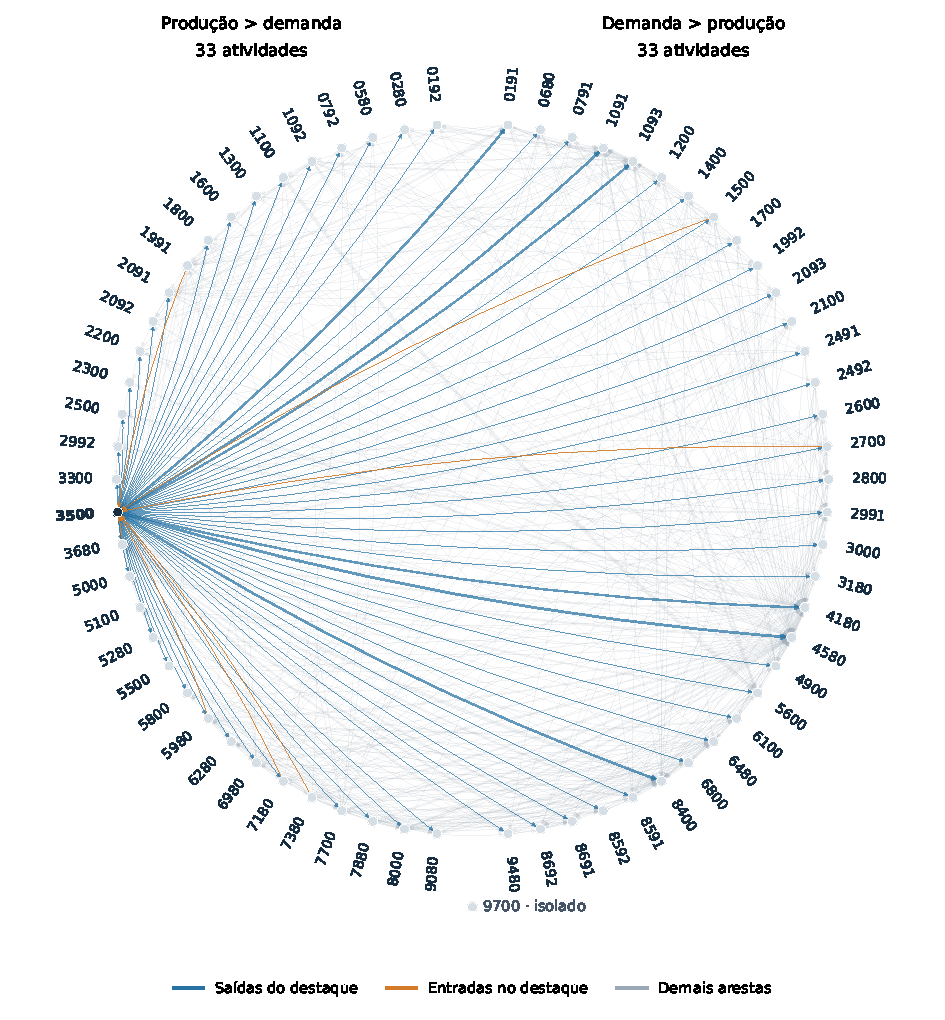
\includegraphics[width=\textwidth,height=0.76\textheight,keepaspectratio]{figuras/rede_foco_3500.pdf}
\caption{Duas perspectivas do mesmo backbone: (a) destaque para energia (3500).}
\label{fig:rede-focos}
\begin{minipage}{\textwidth}\footnotesize
Fonte: elaboração própria. Cada vista mantém 67 nós e 575 arestas em $\alpha=0{,}05$. Azul: saídas do destaque; laranja: entradas; cinza: demais arestas. Energia tem 62 saídas e sete entradas, com cobertura de 99,2\% e 42,1\% do volume externo de cada direção. Área dos nós uniforme; espessura cresce com a raiz quadrada do peso. Posição definida pelo sinal de $u-c$ e pela ordem IBGE: 33 nós com $c>u$ à esquerda, 33 com $u>c$ à direita e o isolado abaixo. A disposição não resulta de centralidade ou comunidade.
\end{minipage}
\end{figure}
\clearpage
\begin{figure}[p]
\ContinuedFloat
\centering
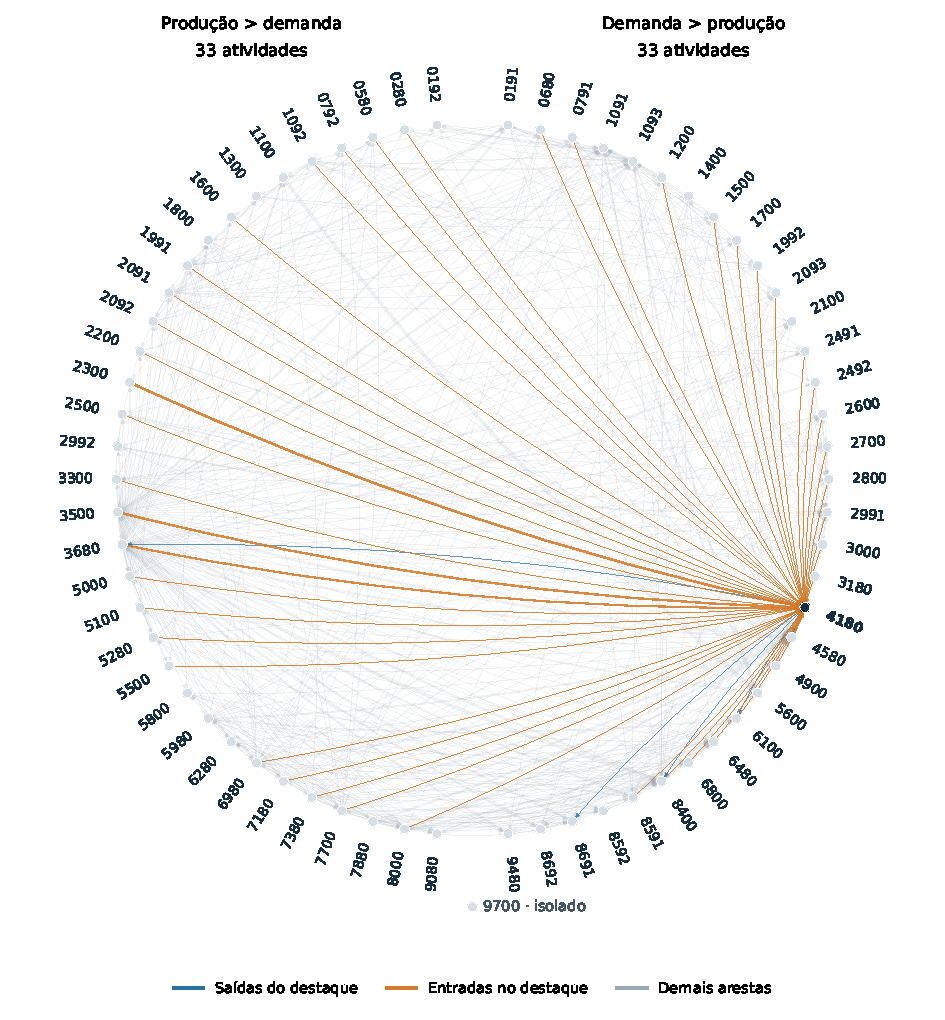
\includegraphics[width=\textwidth,height=0.76\textheight,keepaspectratio]{figuras/rede_foco_4180.pdf}
\caption{Duas perspectivas do mesmo backbone: (b) destaque para construção (4180).}
\begin{minipage}{\textwidth}\footnotesize
Fonte: elaboração própria. Mesmos nós, arestas, posições e escala de espessura do painel (a). Construção tem cinco saídas e 45 entradas, com cobertura de 57,0\% e 91,4\%. Cores representam direção em relação ao destaque, não motivo de retenção. As duas vistas preservam 70,69\% do peso intersetorial de $W$. Cruzamentos e proximidade não representam trajetórias ou distâncias econômicas; relações individuais podem ser consultadas na matriz e nos painéis do anexo.
\end{minipage}
\end{figure}
\clearpage
